\subsection{Motivation}
Der photoelektrische Effekt, dass Licht Elektronen aus Metallen auslösen kann, ist eine Grundlage der Entwicklung der Quantenphysik. Das auftretende Verhalten von Licht lässt sich nicht mehr durch Wellen-, sondern Quanten-/Teilchencharakter erklären. Dass sich unter Bestrahlung die Eigenschaften eines Stoffes ändern (innerer photoelektrischer Effekt), ist Grundlage vieler technologischer Anwendungen von Halbleitern, z. B. bei Lichtsensoren wie CCDs in Kameras, Dioden wie in Solarzellen,... Der äußere photoelektrische Effekt dient z. B. der Oberflächenuntersuchung mit Photoelektronenspektroskopie.

\subsection{Ziele des Versuches}
Durch Experimentieren mit einer Fotozelle wird
\begin{itemize}
    \item die maximale Energie von emittierten Elektronen analysiert
    \item daraus das Planck'sche Wirkungsquantum \(h\) bestimmt
    \item eine Einführung in elektrisch-physikalischen Anwendungen gegeben 
    \item der Durchführende auf die große weite Welt der Wikipedia losgelassen
\end{itemize}
\newpage

\subsection{Technische Grundlagen, Geräte und Durchführung}
Zu den verwendeten Geräten in \cref{fig:Versuchsaufbau.png} gehören:
\begin{enumerate}
    \item Hg-Spektral-Lampe mit Netzteil
    \item Spektrometer mit zwei Prismen und eingebauter Vakuumfotozelle
    \item Gegenspannungsquelle
    \item Strom-Spannungswandler zur Verstärkung des Fotostroms
    \item Multimeter
\end{enumerate}
\begin{table}[htbp]
    \centering 
    \caption{Fehler des Voltmeters je nach gemessener Spannung \(U_I\)}\vspace{0.5cm}
\begin{tabularx}{\textwidth}{cZZZ}
  \toprule
Messbereich & U_I<\qty{0.4}{\volt}  &  \qty{0.4}{\volt}<U_I<\qty{4}{\volt}  & \qty{4}{\volt}<U_I<\qty{40}{\volt} \\ \midrule
Fehler \(\Delta U_I\) [V]     & 0.0025\,U_I+0.0001 & 0.004\,U_I+0.001 & 0.0025\,U_I+0.01\\\bottomrule
\end{tabularx}
\label{table:FehlerVM}
\end{table}

\xfigure{htbp}{scale=0.8}{Versuchsaufbau.png}{Versuchsaufbau\autocite{Skript_1}}{Versuchsaufbau\autocite{Skript_1}}
\clearpage

Der Aufbau ist hier noch mal en Detail zu sehen: 
\begin{figure}[htbp]
  \centering
  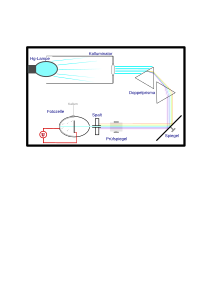
\includegraphics[width=\textwidth]{Zeichnung}
  \caption{Innerer Strahlengang und Funktionsweise des Spektrometers mit Fotozelle}
  \label{fig:Zeichnung}
\end{figure}

Das Licht einer Hg-Gasentladungslampe wird durch einen Kollimator parallelisiert, seine Spektrallinien werden dann durch das Doppelprisma voneinander getrennt und über einen Spiegel auf die Fotokathode (Kalium) gelenkt, je nach Höhe des Spiegels kann eingestellt werden, welche der Spektrallinien durch den Spalt auf die Fotozelle strahlt. Durch einen drehbaren Prüfspiegel kann der Experimentator den Strahl auf ein oberhalb montiertes Ablesepapier lenken (Spaltposition ist dort in einer Flucht markiert), um den Umlenkspiegel entsprechend zu verschieben, damit die Spektrallinie optimal durch den Spalt geht.

Die ausgelösten Elektronen fliegen zum Anodenring und erzeugen einen Fotostrom, der vom Strom-Spannungswandler umgewandelt und verstärkt wird, sodass die Fotospannung \(U_I\) vom Voltmeter gemessen werden kann. Durch eine Gegenspannung \(U\) zwischen Anode und Kathode kann eingestellt werden, welche Elektronen mit welcher kinetischer Energie die Anode erreichen.

\subsection[Theoretische Grundlagen der Physik]{Theoretische Grundlagen der Physik \autocite{Skript_1}}
\subsubsection{Ausschlagen von Elektronen}
Metalle haben eine besondere Bindungsstruktur, die das Herauslösen von Elektronen beeinflusst: Das Metallgitter, die Anordnung der einzelnen Atome, besteht aus positiv geladenen Atomrümpfen, die Valenzelektronen abgegeben haben, dies sind nun die delokalisierten Elektronen, die Leitungselektronen, die sich im Leitungsband frei bewegen können, und dadurch z. B. elektrischen Strom leiten.\\ 
Die Energie der Leitungselektronen eines Metalls wird von der Fermi-Verteilung beschrieben, die von der Temperatur abhängt. Bei \(T = \qty{0}{\K}\) sind alle Energiezustände von Null bis zur Maximalenergie, der Fermienergie \(E_F\) besetzt, d. h. die Wahrscheinlichkeit \(W(E)\), dass sich ein Elektron an einem Zustand (Energieniveau) bis zur Fermienergie befindet, ist (siehe \cref{fig:Fermikante}): 
\[\forall E\leq E_F:\; W(E)= 1\qquad \text{und}\qquad \forall E\geq E_F:\; W(E) = 0.\]
Bei Temperaturen \(T > \qty{0}{\K}\) ist die Fermikante, der Knick bei \(W(E_F)\) aufgeweicht. Das bedeutet, es gibt auch Elektronen mit \(E > E_F\), dafür sind dann aber Energieniveaus darunter unbesetzt. In \cref{fig:energienniveaus} sieht man ein grafisches Modell, wo sich ein Elektron auf dem Energieniveau \(E_e\) im Verhältnis zur Fermienergie befindet.

\begin{figure}[htbp]
\begin{subfigure}[b]{0.48\textwidth}

\includegraphics[height=4cm]{fermikante.png} 
\caption{Aufenthaltswahrscheinlichkeit \(W(E)\) eines Elektrons und Fermikante}
\label{fig:Fermikante}
\end{subfigure}
\hfill
\begin{subfigure}[b]{0.48\textwidth}

\includegraphics[height=4cm]{energienniveaus.png}
\caption{Potentialtopfmodell}
\label{fig:vierleiter}
\end{subfigure}
\caption{Elektronentechnische Grundlagen \autocite{Skript_1}}
\label{fig:energienniveaus}
\end{figure}

Damit ein Elektron nun durch die Energie eines einstrahlenden Photons aus dem Leitungsband ausgelöst werden kann, muss dieses Photon wie in \cref{fig:energienniveaus} eine entsprechende Energie besitzen. Die Energie eines Photons ist frequenzabhängig mit 
\begin{equation}
  E_{\text{Photon}}=h\nu
\end{equation}
Neben der Überwindung des Energieniveauunterschieds \(E_F-E_e\) muss zusätzlich die Austrittsarbeit \(A\) verrichtet werden, eine materialabhängige Größe. Zusätzlich wird auf das Elektron bei ausreichend großer Energie des Photons noch eine kinetische Energiekomponente übertragen. Es folgt also insgesamt:
\begin{equation}
  h\nu=A+(E_F-E_e)+E_{\text{kin}}
\end{equation}
Wenn sich das Elektron nun schon auf einem hohen Energieniveau befindet, am besten sogar \(E_e=E_F\), dann wird alle mögliche Restenergie (\(h\nu-A\)) in kinetische Energie übertragen:
\begin{equation}
  E_{\text{kin}}(\text{max})=h\nu-A
\end{equation}
Das Ziel des Aufbaus mit der Fotozelle und der angelegten Gegenspannung ist es, für jede der Spektrallinien der Hg-Lampe die elektrische Energie \(E_{\text{el}}\) zu variieren, bis keine Elektronen mehr die Anode erreichen, d. h. die kinetische Energie genau gleich der elektrischen Energie ist. Ist also der Fotostrom \(U_I\), der über Anode und Kathode gemessen wird, null, so ist:
\[E_{\text{kin}}=E_{\text{el}}\]
\begin{equation}
  h\nu-A=e U_S
  \label{eq:hs}
\end{equation}
mit der Elementarladung \(e\) und der Sperrspannung \(U_S\) des Gegenspannungsfeldes. Es gelangen also alle Elektronen zur Anode, für die gilt: 
\begin{equation}
  E_F-E_e<h\nu-A-eU
  \label{eq:Bedingung}
\end{equation}
Da \(W(E)=1\) für alle Energieniveaus bei \(T = \qty{0}{\K}\), werden also bei einer gewissen Gegenspannung eine gewisse Anzahl an \(n\) Elektronen ausgelöst, für die die Bedingung \cref{eq:Bedingung} gilt. Damit ist der Fotostrom \(I=\frac{ne}{t}\) proportional zu \(U\) (da \(n\sim U\)). 
Dies gilt nur für \(T = \qty{0}{\K}\)! Wie oben erwähnt gibt es unter realen Bedingungen auch Elektronen mit \(E_e>E_F\), uns interessiert aber nur der annähernd konstante Anteil von \(W(E)=1\) in \cref{fig:Fermikante}, deswegen messen wir keinen linearen Abfall von \(U_I\) bei Variation von \(U\), da \(W(E)\neq 1\) für \(eU\rightarrow E_{\text{kin}}(\text{max})\).  
Das heißt wir variieren zur Bestimmung von der Sperrspannung \(U_S\) die Gegenspannung \(U\) solange, bis der am Multimeter gemessene Fotostrom annähernd null wird. Durch eine große Range von \(U\) stellen wir sicher, dass auch ein linearer Verlauf von \(U_I(U)\) gemessen wird, für den \(W(E)=1\) gilt. \\
Die paar hochenergetischen Elektronen interessieren uns nicht, denn diese brechen das lineare Verhältnis von \(U_I\sim U\).

Jedoch muss man noch einen zweiten Effekt betrachten, außer der Nichtlinearität für hohe kinetische Energien: Durch die Geometrie der vorliegenden glühbirnenförmigen Fotozelle gilt:
\[\sqrt{U_I}\sim U\]
Der dritte Effekt der betrachtet werden muss, bis \(\sqrt{U_I}(U)\) aufgetragen werden kann, ist dass durch Kalium, welches sich auf der Anode niedergeschlagen hat, bei egal welcher Gegenspannung auch ein Fotostrom (Untergrundstrom) \(U_{I_0}\) direkt an der Anode entsteht, der in entgegengesetzte Richtung fliegt. Dieser muss also noch vom eigentlich gewollten Kathodenfotostrom \(U_I\) abgezogen werden (er wird bei hoher negativer Gegenspannung erhoben, d. h. \(U_{I_0}<0\), deswegen das Subtrahieren, man könnte auch \(U_I'=U_I+|U_{I_0}|\) schreiben).\\
Final wird also aufgetragen, zur Bestimmung der Sperrspannung durch Extrapolation des linearen Verhaltens von: 
\begin{equation}
    \sqrt{U_I-U_{I_0}}(U)
\end{equation}

\subsubsection{Spektrallinien}
Befindet sich ein Elektron auf einem höheren Energieniveau, z. B. durch anregende elektrische Energie wie in der Quecksilber(Hg)-Gasentladungslampe, kommt es auch irgendwann wieder zu einem Quantensprung auf ein niedrigeres Energieniveau. Dabei wird die Differenz der zwei Energieniveaus durch Abstrahlung von Photonen frei, die genau die Energie der Differenz der zwei quantenmechanischen Zustände besitzen, d. h. es wird eine Lichtwelle emittiert, die eine bestimmte Frequenz bzw. Wellenlänge hat. Diese Emission passiert meist spontan. Für bestimmte Übergänge zwischen Energieniveaus, die je nach Atom anders sind, gibt es also charakteristische Frequenzen (Energie eines Photons \(E_p=h\nu\)), mit dem Planckschen Wirkungsquantum \(h\) und der Frequenz \(\nu\) bzw. Wellenlängen. Trägt man dieses Spektrum auf, so sieht man die Spektrallinien eines Stoffes. Die Emissionslinien (Elektron fällt von einem anregenden Zustand zurück) sehen wir bei den verwendeten Gasentladungslampen.

Die Frequenzen der untersuchten Spektrallinien finden sich hier:
\begin{table}[htbp]
  \centering
  \caption{Klassifizierung der untersuchten Spektrallinien \autocite{Skript_1}}
\begin{tabularx}{0.8\textwidth}{cTTTTT}
\toprule
Farbe  & UV    & Violett & blau  & grün  & gelb  \\ \midrule
\(f\;[\unit{\tera\hertz}]\) & 821.3 & 740.2    & 687.9 & 549.0 & 518.7\\
\bottomrule
\end{tabularx}
\label{table:frequenzen}
\end{table}